\chapter{Pickup Ions} % Main chapter title

\label{chapter:theory} % For referencing the chapter elsewhere, use \ref{Chapter1} 

%-------------------------------------------------------------



%-------------------------------------------------------------

%Pickup ions are created when neutral atoms inside the heliosphere become ionised and are subsequently swept away with the heliospheric magnetic field that is embedded within the solar wind.
A neutral atom inside the heliosphere is only subjected to the gravitational force and radiation pressure of the Sun. It is not sensitive to any electromagnetic forces until it becomes ionized by solar ultra-violet radiation, charge exchange with solar wind protons or electron impact \citep{rucinsky}. After ionization the particle starts interacting with the solar wind plasma. In particular it is forced onto a gyro orbit about the heliospheric magnetic field that is embedded within the solar wind. As the freshly created ion is swept away with the magnetic field line it is ``picked up'' from its location of ionization -- a new pickup ion (PUI) has been created.
\\ \\
PUI are mostly only singly charged. This characteristic can help to distinguish them from solar wind ions of coronal origin which often have been ionized multiple times, if not completely. Additionally, PUI are characterized by a broad, non-Maxwellian Velocity Distribution Function. This is formed by the pickup process and the following interaction with the magnetized solar wind plasma, which will be described in more detail in Sec. \ref{sec:theo_vdf}.\\
PUI were observed for the first time by \citet{moebius_nature_85} as $\mathrm{He^{+}}$ with the SULEICA Instrument on the AMPTE spacecraft at $1\,\mathrm{AU}$. Since then, a variety of other PUI species like $\mathrm{H^{+}}$, $\mathrm{He^{2+}}$ or $\mathrm{C^{+}}$, $\mathrm{N^{+}}$, $\mathrm{O^{+}}$, $\mathrm{Mg^{+}}$, $\mathrm{Si^{+}}$ and $\mathrm{Fe^{+}}$ has been observed.\\
There are two possible origins for the PUI's neutral seed population. One of them is the interstellar medium, the other a source inside the heliosphere.
\section{Interstellar Pickup Ions}
The heliosphere can be imagined as a big bubble that is blown up by the solar wind and confined by the heliopause. This bubble is embedded in the Local Interstellar Medium (LISM), which moves with a velocity of $\sim 25\,\mathrm{km\,s^{-1}}$ relative to the heliosphere. As the LISM is a relatively cold plasma with $T_{LISM} \sim 7000\,\mathrm{K}$ \citep{frisch}, it is not completely ionized. The neutral part of the LISM can enter the heliosphere as it is not deflected by the heliosheath. Due to the relative motion of the LISM against the heliosphere, a continuous stream of neutral particles enters the heliosphere.\\
Inside the heliosphere the neutrals are guided only by the gravitational force and radiation pressure of the Sun. The neutral particle's species determines how deep it can travel into the heliosphere before it becomes ionized. Species with a higher First Ionization Potential will be able to approach the Sun much further without being ionized \citep{kallenbach_2000}. This results in $\mathrm{He^{+}}$ being the dominant PUI species at a solar distance of $1\,\mathrm{AU}$ even if in the LISM the abundance of $\mathrm{H}$ is about ten times the one of $\mathrm{He}$ \citep{frisch}.
\section{Inner-source Pickup Ions}
The idea of an additional source for the PUI's neutral seed population was born when \citet{geiss_1995a} measured a global distribution of $\mathrm{C^{+}}$ PUI with the SWICS instrument on Ulysses.  Interstellar $\mathrm{C}$ exists almost exclusively in a singly charged state \citep{Frisch} in the LISM. As only neutral atoms can enter the heliosphere it was not expected to find a significant signature of $\mathrm{C^{+}}$ PUI. However, PUI $\mathrm{C^{+}}$ was observed with about the same ratio as $\mathrm{O^{+}}$ PUI, of which, in contrast, ~80\% is in a neutral charge state in the interstellar medium. These findings suggested that there must be another source for neutrals that has its origin somewhere inside the heliosphere. In following studies \citep[e.g.][]{geiss_1995b} there were found also other species like $\mathrm{O^{+}}$ and $\mathrm{Ne^{+}}$ of these, so called, inner-source PUI.\\
Inner-source PUI show a composition that is similar to the one of the solar wind \citep{gloeckler2000_innersource, allegrini_2005} as well as a VDF that is centered around $w_{\mathrm{sc}} \approx 1$ \citep{schwadron_2000} and seems to have thermalized with the solar wind.
\\
However, inner-source PUI are not completely understood until today. In particular the production mechanism of their neutral seed population is under debate. \citet{allegrini_2005} have summarized current candidates for possible scenarios. Two of those give an explanation for the ions' composition as they directly incorporate solar wind ions in the process:
\begin{itemize}
	\item Solar wind recycling \citep{gloeckler2000_innersource, schwadron_2000}: Absorption of solar wind ions by heliospheric grains and subsequent reemission of neutral atoms
	\item Solar wind neutralization \citep{wimmer_2002}: Solar wind ions penetrate sub-micron-sized dust grains and undergo (partial) neutralization by charge exchange
\end{itemize}
However, as this work does not focus on inner-source PUI in particular and as we do not know their production mechanism for certain, the following considerations mainly relate to interstellar PUI.
%
%
%
\section{Pickup Ion Velocity Distribution Function}
\label{sec:theo_vdf}
For understanding the initial shape of the PUI VDF one needs to consider the pickup process itself. \\
For neutrals from the LISM their initial speed $v_{\mathrm{ini}}$ before being ionized is mainly given by the inflow speed $v_{\mathrm{LISM}}$ of the local interstellar medium with which they enter the heliosphere. \citet{schwadron_2015_ibex} obtained $v_{\mathrm{LISM}} \approx 25 \,\mathrm{km\,s^{-1}}$ for $\mathrm{He}$ with the IBEX satellite. Considering the acceleration by the Sun's gravitational force we have a maximum initial speed of $v_{\mathrm{ini}} \approx 50 \,\mathrm{km\,s^{-1}}$ at $1\,\mathrm{AU}$. Compared to an average solar wind speed of $v_{\mathrm{sw}} \approx 400\,\mathrm{km\,s^{-1}}$ one can neglect this initial speed in a first step. For simplicity we thus consider a neutral particle at rest that becomes ionized by one of the aforementioned processes. The freshly created ion is now subjected to the electromagnetic forces of the solar wind plasma. In particular, it finds itself at a velocity $v_{\mathrm{sw}}$ relative to the magnetic field which is convected outwards by the solar wind that is assumed to flow radially outwards. Due to the Lorentz force the PUI starts to gyrate about the magnetic field line on an orbit that is perpendicular to the field line.
When we further consider a magnetic field's orientation that is perpendicular to the solar wind flow, $\vec{B} \perp \vec{v}_{\mathrm{sw}}$, the ion's gyration speed is $v_{\mathrm{sw}}$ while its guiding center moves together with the field line at a speed of $v_{\mathrm{sw}}$ as well.
Thus, the total speed of the PUI ranges between $0\, \mathrm{v_{\mathrm{sw}}} $ and $2 \, \mathrm{v_{\mathrm{sw}}}$ in a Sun frame of reference, s. Fig. \ref{fig:pu_proc}.
\begin{figure}[h]
	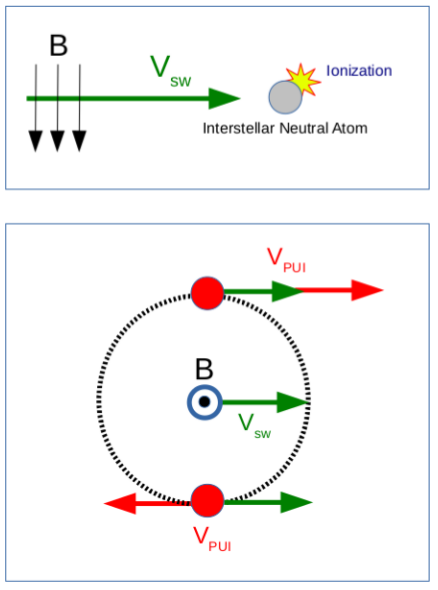
\includegraphics[width=0.4\textwidth]{Figures/pu_process_1_2.png}
	\centering
	\caption{Visualization of the pickup process. We assume a neutral particle at rest and a magnetic field moving perpendicular to the solar wind and at solar wind speed relative to the particle (upper panel). Being ionized in this situation, the particle is forced onto a gyro-orbit about the magnetic field line. The ion's total velocity then ranges from $0\, \mathrm{v_{\mathrm{sw}}} $ to $2 \, \mathrm{v_{\mathrm{sw}}}$ in a Sun frame of reference (lower panel). The figure is taken from \citet{talk_etss}.}
	\label{fig:pu_proc}
\end{figure}
As the heliospheric magnetic field lines are shaped like an Archimedean spiral, the so-called ``Parker Spiral'', the assumption of a perpendicular magnetic field only applies when solar wind speed $v_{sw}$ and solar distance $r_\odot$ follow the relation
\begin{align*}
90 ^\circ \approx  \arctan \left( \frac{2\pi}{T_\odot \cdot v_{\mathrm{sw}}} r_\odot \right)
\end{align*}
with the Sun's sidereal period $T_\odot \approx 25\,\mathrm{d}$ \citep{prlss_2004}.
In other cases, e.g. for solar distances about $1\,\mathrm{AU}$, at which the angle between solar wind and magnetic field direction is approximately $45^\circ$, the maximum speed in a Sun frame of reference is decreased.
However, independent of the magnetic field orientation, every possible velocity space trajectory is part of a spherical shell with the radius $v_{\mathrm{sw}}$ centered around $\vec{v}_{\mathrm{sw}}$. That means that, in the frame of the solar wind, the freshly created PUI always moves with a speed that is as fast as the solar wind itself.
\\
Instead of a single PUI we can consider an ensemble of PUI that is injected into the solar wind while the magnetic field orientation is not changing significantly. In this scenario we expect the VDF to form a ring shape in velocity space, commonly called the ``PUI torus VDF'' \citep{oka_2002}. The expected orientation of this highly anisotropic VDF depends on the local magnetic field direction and is sketched in Fig.~\ref{fig:pu}, left panel, for a magnetic field direction that is slightly tilted from a perpendicular direction relative to the solar wind.
\begin{figure}
	\centering
	\begin{subfigure}{.32\textwidth}
		\centering
		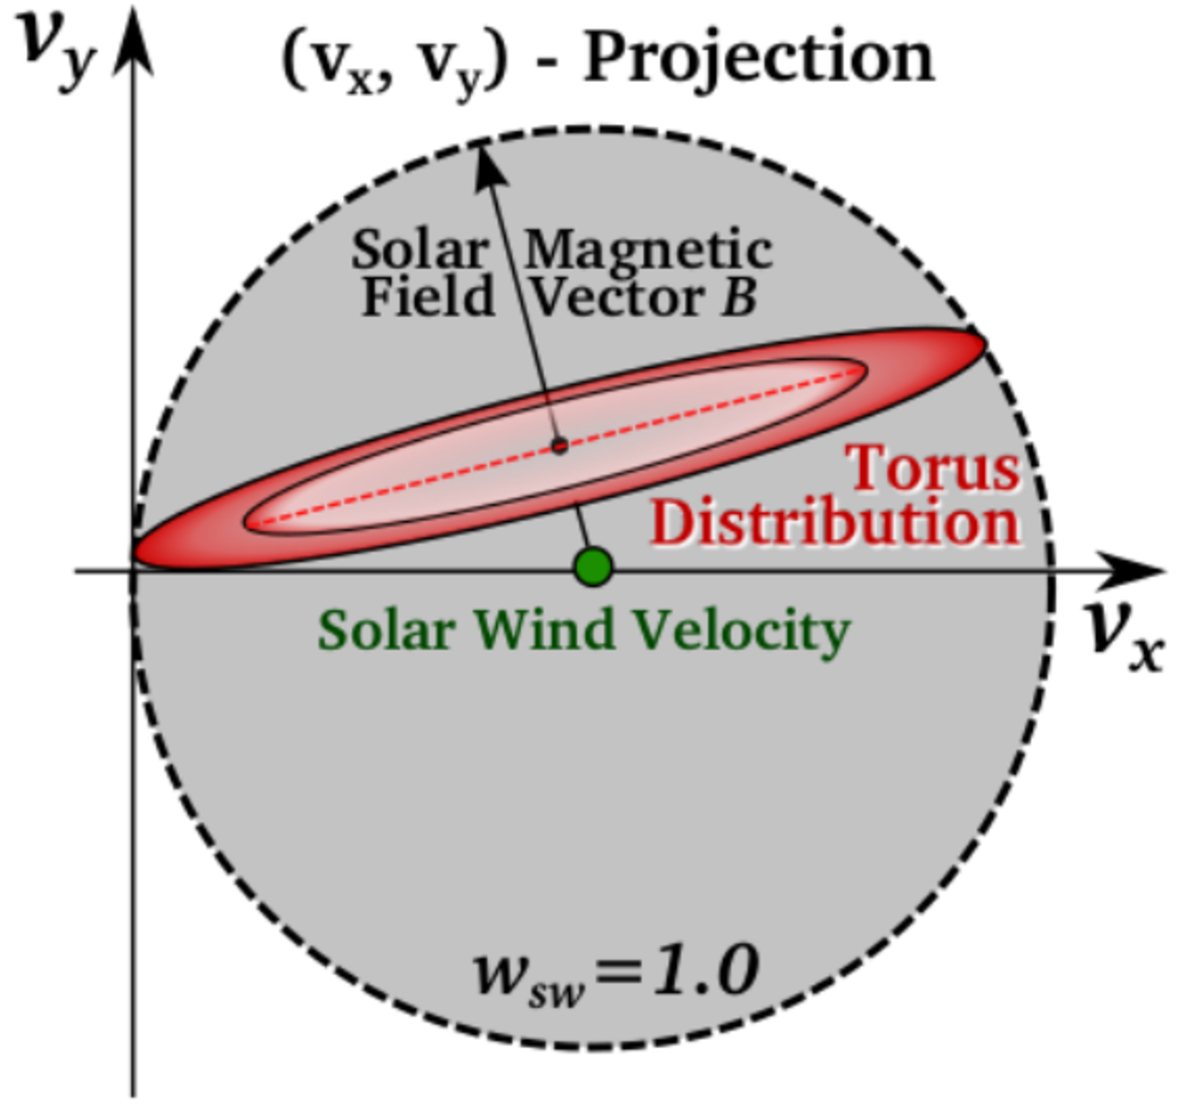
\includegraphics[width=1.\linewidth]{Figures/torus.pdf}
	\end{subfigure}%
	\begin{subfigure}{.32\textwidth}
		\centering
		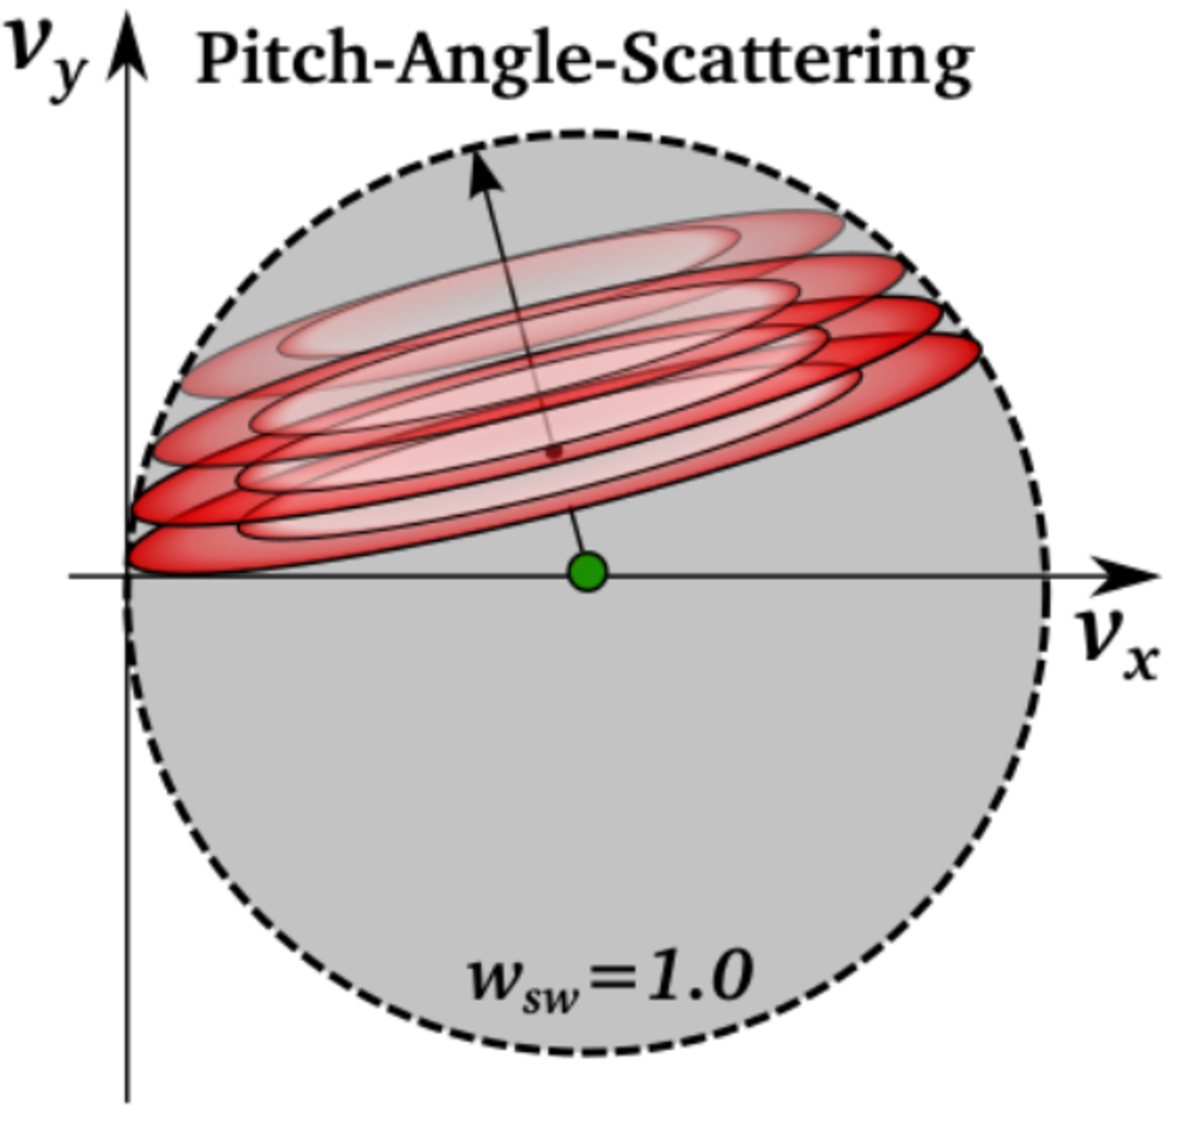
\includegraphics[width=1.\linewidth]{Figures/PAS.pdf}
	\end{subfigure}
	\begin{subfigure}{.32\textwidth}
		\centering
		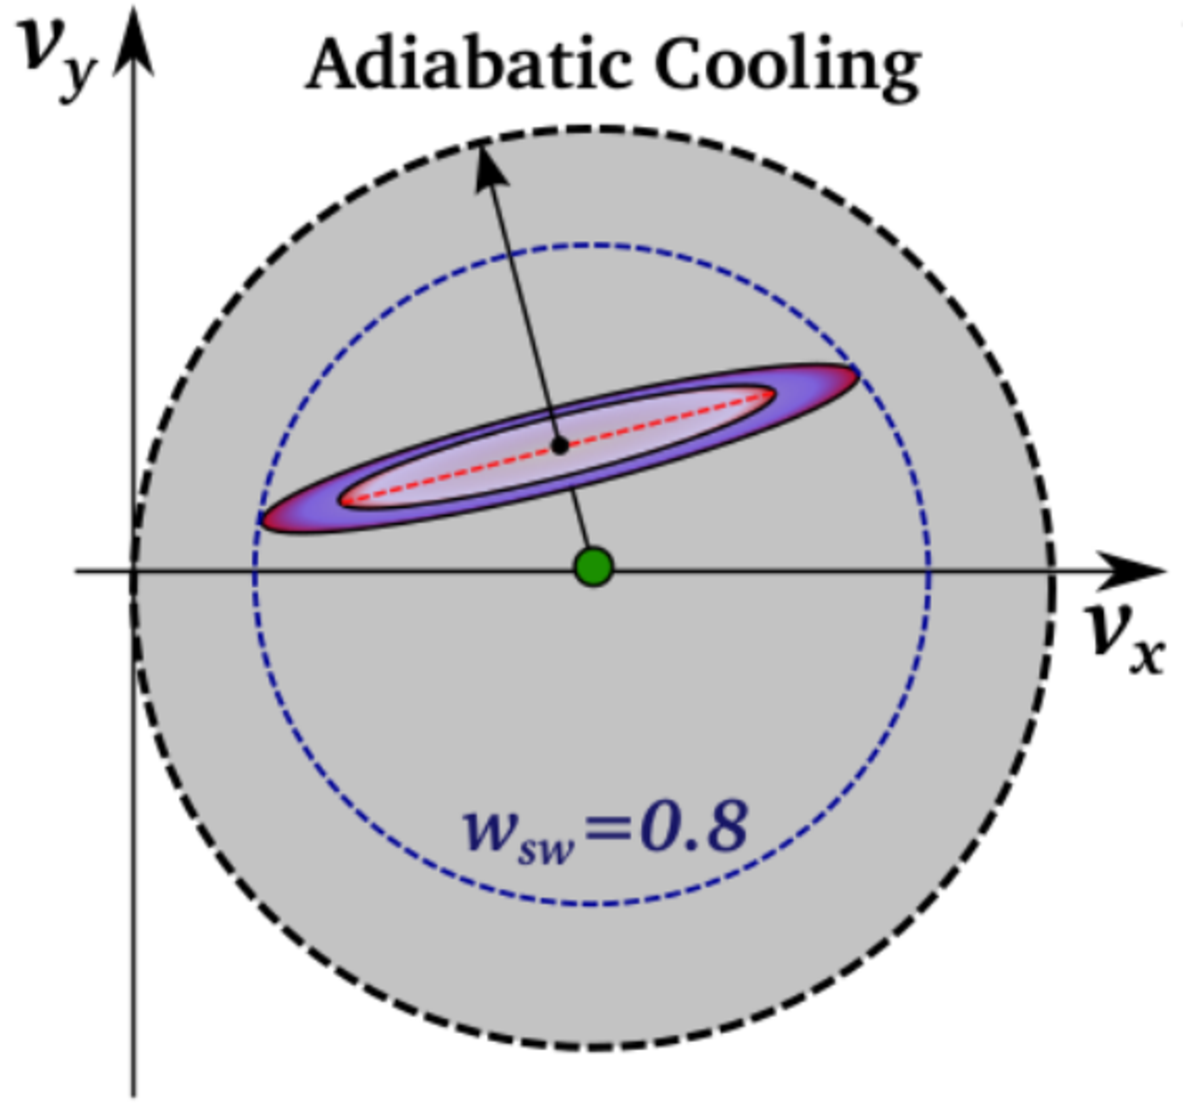
\includegraphics[width=1.\linewidth]{Figures/Cooling.pdf}
	\end{subfigure}
	\caption{Velocity space diagrams for an initial PUI torus distribution (left), the same distribution under the influence of pitch-angle scattering (center) and after the distribution has been ``cooled'' (right). For a better visibility of the torus character the $v_x-v_y$ plane is slightly tilted. The figure is from \citet{drews_2015}, modified.}
	\label{fig:pu}
\end{figure}
After the injection, the PUI population is radially carried away with the solar wind. During phase space transport through the heliosphere the PUI are subjected to multiple processes that are expected to modify the shape of the initial toroidal VDF. However, it is not completely understood how the VDF evolves in detail.
\\
A fast isotropization of the VDF due to pitch-angle scattering was suggested by \citet{vasyl_siscoe_1976} in a theoretical work. This would result in a VDF that is distributed across the complete surface of the spherical shell with radius $v_{\mathrm{sw}}$. Fig. \ref{fig:pu}, center, shows the initial influence of pitch-angle scattering. \\
However, observations by e.g. \citet{moebius_98} on $\mathrm{He^{+}}$ or \citet{gloeckler_1995} on $\mathrm{H^{+}}$ have shown clear anisotropic features in the measured VDF. Following studies \citep[e.g.][]{isenberg} tried to explain these findings with the assumption that the ions would be injected more likely into the sunward hemisphere of velocity space. Ineffective pitch-angle scattering into the antisunward hemisphere would thus result in a radial anisotropy.
\\
Recent observations have emphasized the influence of the magnetic field direction on the measured anisotropy. Utilizing 2D analyses of the velocity space, \citet{oka_2002} and \citet{drews_2015} found that the measured VDF of PUI is systematically oriented around the direction that is perpendicular to the magnetic field. Thus, it is believed that the VDF's anisotropic features are remnants of the initial toroidal VDF as the pitch-angle scattering is not as effective as assumed originally.\\
Furthermore, there are different acceleration and deceleration processes that change the PUI's initial VDF and lead to a diffusion in velocity space. The general idea of a toroidal distribution that has undergone some deceleration is shown in Fig.~\ref{fig:pu}, right.\\
Under the assumption of an isotropic VDF the PUI population is often treated as an adiabatic gas that is consequently ``cooled'' when expanding with the solar wind \citep{vasyl_siscoe_1976}. Another cooling mechanism, called the \textit{magnetic cooling}, is due to the magnetic field weakening with solar distance. When the PUI are swept outwards both their magnetic moment and their ``Complex Ginzburg-Landau invariant'' \citep{fahr} have to be conserved. This leads to a decrease in both velocity components (parallel and perpendicular to the magnetic field) and thus to a decrease in total velocity in the frame of the solar wind. For a more detailed description of these effects see e.g. \citet{fahr_fichtner}.\\
However, all of these theories assume an isotropic PUI VDF and thus must be reviewed carefully.\\
Acceleration of PUI can be caused by several processes. Among those are interplanetary shock waves resulting from Coronal Mass Ejections or Stream Interaction Regions, that are generally known as drivers for particle acceleration in the heliosphere \citep[Ch. 7.5]{kallenrode}. Additional possible mechanisms, including the ``pump acceleration'', are described in \citet{fisk_gloeckler2012}. Just as the aforementioned cooling processes the acceleration of PUI is still not completely understood.